\documentclass{standalone}
%\usepackage{mathpazo}
\usepackage{tikz}

\usetikzlibrary{arrows}
\usetikzlibrary{decorations.markings}

\begin{document}
    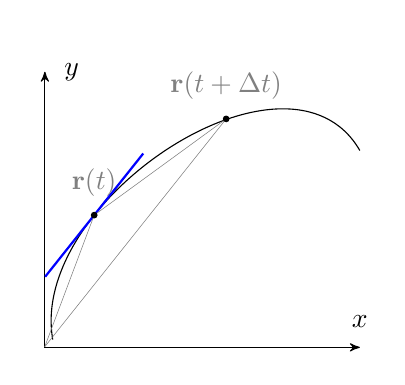
\begin{tikzpicture}[
    tangent/.style={
        decoration={
            markings,% switch on markings
            mark=
            at position #1
            with    {
                \coordinate (tangent point-\pgfkeysvalueof{/pgf/decoration/mark info/sequence number}) at (0pt,0pt);
                \coordinate (tangent unit vector-\pgfkeysvalueof{/pgf/decoration/mark info/sequence number}) at (1,0pt);
                \coordinate (tangent orthogonal unit vector-\pgfkeysvalueof{/pgf/decoration/mark info/sequence number}) at (0pt,1);
        }  },
        postaction=decorate
    },
    use tangent/.style={
        shift=(tangent point-#1),
        x=(tangent unit vector-#1),
        y=(tangent orthogonal unit vector-#1)
    },
    use tangent/.default=1
    ]
    
    \draw [<->,>=stealth'] (0,3.5) node [label = right:{$y$}]{} -- (0,0) -- (4,0) node[label = above:{$x$}]{};
    \draw [  tangent=0.3 ] (0.1,0.1)  to [out=100,in=120] (4,2.5);
    \draw [blue, thick, use tangent] (-1,0) -- (1,0);
    \draw [use tangent, help lines](0,0)node[label=above:{ ${\bf r}(t)$}]{}--(-1.7,-0.55);
    \draw [use tangent, help lines](-1.7,-0.55)--(2,-0.55)node[label=above:{ ${\bf r}(t+\Delta t)$}]{};
    \draw [use tangent, help lines](0,0)--(2,-0.55);
    \filldraw[use tangent] (0,0) circle (1pt);
    \filldraw[use tangent] (2,-0.55) circle (1pt);
\end{tikzpicture}
\end{document}